% This file was created by tikzplotlib v0.9.8.
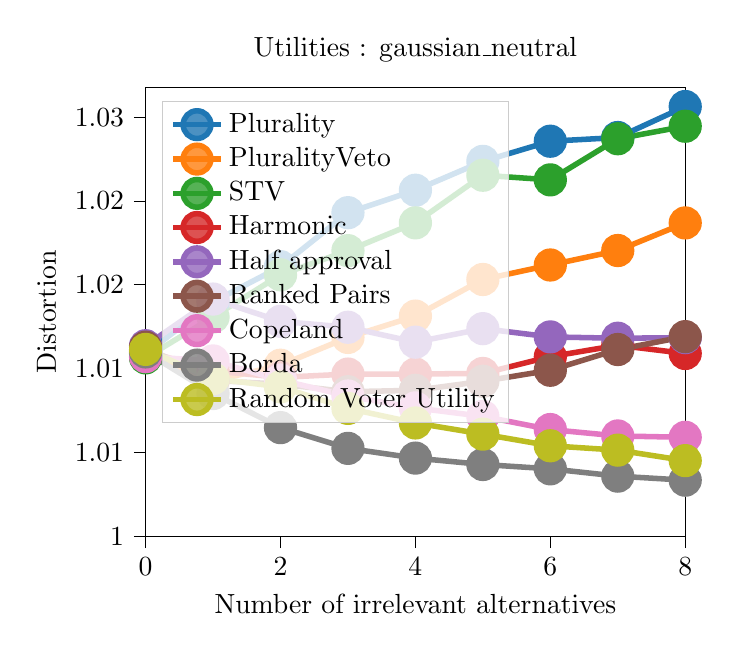
\begin{tikzpicture}

\definecolor{color0}{rgb}{0.12156862745098,0.466666666666667,0.705882352941177}
\definecolor{color1}{rgb}{1,0.498039215686275,0.0549019607843137}
\definecolor{color2}{rgb}{0.172549019607843,0.627450980392157,0.172549019607843}
\definecolor{color3}{rgb}{0.83921568627451,0.152941176470588,0.156862745098039}
\definecolor{color4}{rgb}{0.580392156862745,0.403921568627451,0.741176470588235}
\definecolor{color5}{rgb}{0.549019607843137,0.337254901960784,0.294117647058824}
\definecolor{color6}{rgb}{0.890196078431372,0.466666666666667,0.76078431372549}
\definecolor{color7}{rgb}{0.737254901960784,0.741176470588235,0.133333333333333}

\begin{axis}[
legend cell align={left},
legend style={
  fill opacity=0.8,
  draw opacity=1,
  text opacity=1,
  at={(0.03,0.97)},
  anchor=north west,
  draw=white!80!black
},
tick align=outside,
tick pos=left,
title={Utilities : gaussian\_neutral},
x grid style={white!69.0196078431373!black},
xlabel={Number of irrelevant alternatives},
xmin=0, xmax=8,
xtick style={color=black},
y grid style={white!69.0196078431373!black},
ylabel={Distortion},
ymin=1, ymax=1.02674396736415,
ytick style={color=black}
]
\addplot [line width=2pt, color0, mark=*, mark size=5, mark options={solid}]
table {%
0 1.01087860312474
1 1.0139754447308
2 1.01607873527441
3 1.0192991156025
4 1.02063815767279
5 1.02236011569123
6 1.02356159434541
7 1.02378247110008
8 1.02562953438811
};
\addlegendentry{Plurality}
\addplot [line width=2pt, color1, mark=*, mark size=5, mark options={solid}]
table {%
0 1.01094184054347
1 1.00926137004537
2 1.01019913390888
3 1.01185792167371
4 1.01312925107057
5 1.01531333643269
6 1.01617827415259
7 1.01704182126692
8 1.01868811813238
};
\addlegendentry{PluralityVeto}
\addplot [line width=2pt, color2, mark=*, mark size=5, mark options={solid}]
table {%
0 1.01063741115765
1 1.0130765429981
2 1.01559327510448
3 1.0170333861666
4 1.01869287402003
5 1.02153268716982
6 1.02125611398063
7 1.02370948655109
8 1.02445590115668
};
\addlegendentry{STV}
\addplot [line width=2pt, color3, mark=*, mark size=5, mark options={solid}]
table {%
0 1.01105602437933
1 1.00986136626399
2 1.0094760635147
3 1.00967040300955
4 1.00967534863634
5 1.00970801471809
6 1.01071110898548
7 1.01138824331318
8 1.01089981941465
};
\addlegendentry{Harmonic}
\addplot [line width=2pt, color4, mark=*, mark size=5, mark options={solid}]
table {%
0 1.0113627923843
1 1.01414599787916
2 1.01281685819801
3 1.01246396181042
4 1.01157419555585
5 1.01238073096044
6 1.01188766013099
7 1.01180927690563
8 1.01184471429306
};
\addlegendentry{Half approval}
\addplot [line width=2pt, color5, mark=*, mark size=5, mark options={solid}]
table {%
0 1.0112754682586
1 1.00929633544891
2 1.00906855398354
3 1.00861911006816
4 1.00870201669024
5 1.00924137251732
6 1.00989891137396
7 1.01113578685719
8 1.01190429160979
};
\addlegendentry{Ranked Pairs}
\addplot [line width=2pt, color6, mark=*, mark size=5, mark options={solid}]
table {%
0 1.01070999174075
1 1.01045559164336
2 1.00931393825882
3 1.00836124081109
4 1.00765352996446
5 1.00714750302556
6 1.00636175636519
7 1.00597994322815
8 1.00589949424024
};
\addlegendentry{Copeland}
\addplot [line width=2pt, white!49.8039215686275!black, mark=*, mark size=5, mark options={solid}]
table {%
0 1.01099123922715
1 1.00851117525779
2 1.00647742962352
3 1.00523892380435
4 1.00465841514023
5 1.00427688834267
6 1.00401773854981
7 1.0035818667938
8 1.00334087486726
};
\addlegendentry{Borda}
\addplot [line width=2pt, color7, mark=*, mark size=5, mark options={solid}]
table {%
0 1.0111420490065
1 1.00940163103382
2 1.00890926624714
3 1.00762391210668
4 1.00675511923754
5 1.00608912126246
6 1.00539348139452
7 1.00513362730322
8 1.00450836669973
};
\addlegendentry{Random Voter Utility}
\end{axis}

\end{tikzpicture}
